\section{Описание сервера сбора данных}

ССД обслуживает низкоуровневое взаимодействие с УСПД. После получения данных этот блок передает информацию модульной системе драйверов. Система драйверов осуществляет взаимодействие на верхнем уровне модели OSI. За счет модульности обеспечивается расширение парка поддерживаемого оборудования. Также ССД содержит систему управления сетью и взаимодействия с базой данных: он осуществляет контроль работоспособности сети, выполняет отбраковку данных, отвечает за принятие решений о повторном запросе на сбор данных, классифицирует информацию, обеспечивает контроль единого времени и осуществляет запись информации в базу данных.

Логически ПО ССД можно разделить на 3 блока, каждый из которых выполняет отдельную задачу:
\begin{enumerate}
\item блок контроля приема и передачи данных, который отвечает за взаимодействие ССД с УСПД/УУ;
\item временная база данных (ВБД). В ходе проектирования ПО ССД было рассмотрено два варианта обработки и записи данных с УСПД/УУ на СБД: 
\begin{itemize}
\item обработка и запись данных на СБД по мере их поступления от УСПД/УУ;
\item запись поступающих данных в ВБД и последующая обработка и передача на СБД.
\end{itemize}
\item блок обработки данных.
\end{enumerate}

Использование первого варианта может привести к потере данных, так как вновь поступающие данные не будут успевать обрабатываться ПО ССД. Второй вариант позволяет обеспечить целостность поступивших данных, поэтому он является более предпочтительным.

Обобщенная функциональная схема функционирования ПО ССД представлена на рисунке \ref{sh_ssd:sh_ssd}.

\begin{figure}[h!]
 \center{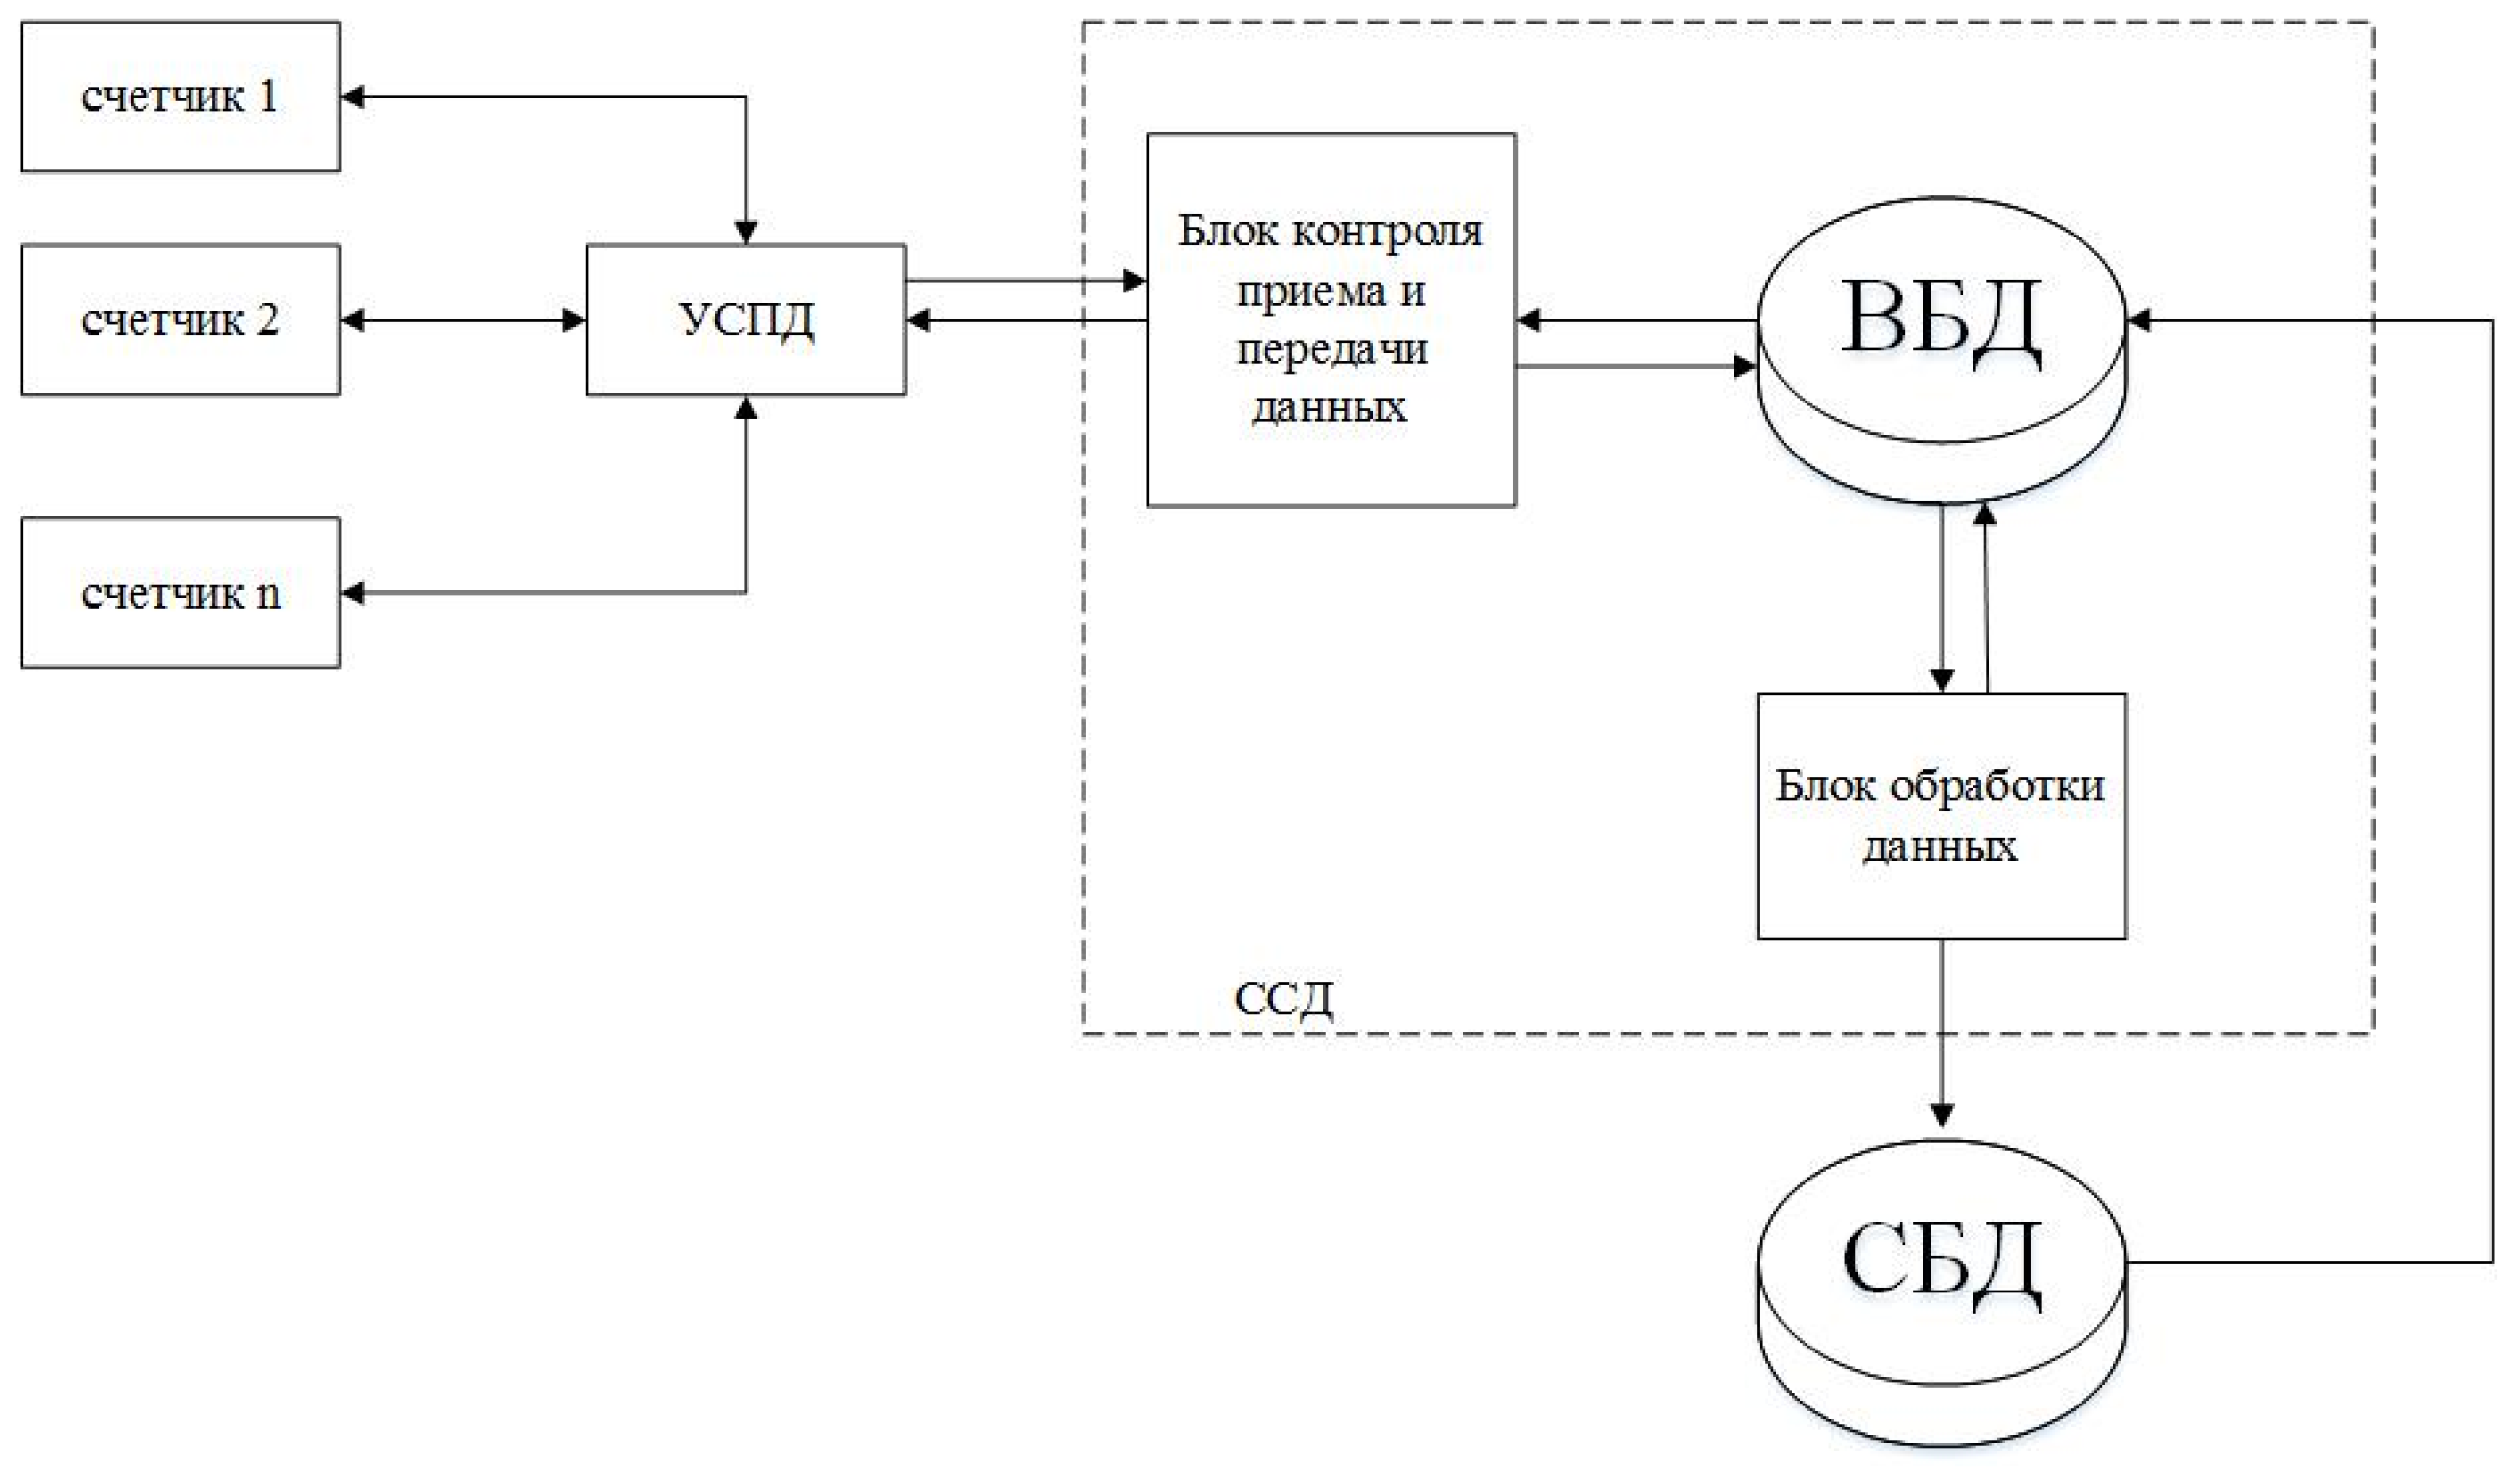
\includegraphics[width=0.8\linewidth]{sh_ssd}}
 \caption{Функциональная схема ССД}
 \label{sh_ssd:sh_ssd}
\end{figure}
